\documentclass[11pt]{article}
\usepackage[a4paper,margin=1in]{geometry}
\usepackage{amssymb,mathtools}
\usepackage{booktabs}
\usepackage{graphicx}
\usepackage[T1]{fontenc}
\usepackage{lmodern}
\usepackage{listings}
\usepackage{subcaption}
\usepackage{float}
\usepackage[utf8]{inputenc}
\usepackage{hyperref}

\lstset{
  basicstyle=\ttfamily\small,
  keywordstyle=\color{blue!60!black},
  commentstyle=\color{green!40!black},
  stringstyle=\color{red!60!black},
  showstringspaces=false,
  frame=single,
  breaklines=true,
  tabsize=2
}

\title{Comp 480/580 --- Assignment \#1}
\author{Dev Sanghvi - ds221}
\date{Rice University \\ Date: 09/30/2025}

\begin{document}
\maketitle

\section*{Constants}
\begin{itemize}
  \item \textbf{Global seeds}: \verb|SEED_COEFFS = 580123|, \verb|SEED_KEYS = 20250916|, \verb|SEED_BLOOM = 137|.
  \item \textbf{Prime} \(P = 1{,}048{,}573\).
  \item \textbf{Fixed coefficients} (drawn once with \verb|SEED_COEFFS| and then \emph{frozen}):
  \[
    a=716{,}663,\quad b=625{,}113,\quad c=32{,}912,\quad d=480{,}811.
  \]
\end{itemize}

\newpage
\section{Testing Hash Functions }
\textbf{Goal} Check for the avalanche behavior: for 31 input bits and 10 output bits, estimate the probability \(P[\text{output bit } i \text{ flips} \mid \text{input bit } j \text{ flips}]\)
for each of four hash families:
\begin{align*}
  h_1(x) &= \big((ax + b) \bmod P\big) \bmod 1024 \quad (\text{2-universal}),\\
  h_2(x) &= \big((ax^2 + bx + c) \bmod P\big) \bmod 1024 \quad (\text{3-universal}),\\
  h_3(x) &= \big((ax^3 + bx^2 + cx + d) \bmod P\big) \bmod 1024 \quad (\text{4-universal}),\\
  h_4(x) &= \texttt{murmurhash3\_32}(x;\,\text{seed}=137) \bmod 1024.
\end{align*}
I generated \(N=5000\) independent 31-bit positive integers \(x\), flip each input bit \(j\in\{0,\ldots,30\}\) to form \(x\oplus 2^j\), compute \(y=h(x), y'=h(x\oplus 2^j)\), and mark whether bit \(i\in\{0,\ldots,9\}\) changed in \(y\oplus y'\). This yields a \(10\times 31\) matrix of empirical probabilities for each hash.

\paragraph{Implementation details} All random sources (\(x\), coefficients) use fixed seeds noted above. MurmurHash3 uses its \texttt{scikit-learn}  implementation.

\paragraph{Summary statistics}
Let \(A\) denote the \(10\times 31\) matrix of probabilities for a hash. I got
\(\text{mean}(A)\), the average absolute deviation from \(0.5\) (AAD), and the min/max entry as follows:

\begin{center}
\begin{tabular}{lcccc}
\toprule
Hash & $\text{mean}(A)$ & AAD from 0.5 & $\min(A)$ & $\max(A)$ \\
\midrule
2-universal      & 0.5352 & 0.2231 & 0.0612 & 0.9692 \\
3-universal      & 0.4997 & 0.0056 & 0.4804 & 0.5224 \\
4-universal      & 0.5000 & 0.0055 & 0.4776 & 0.5170 \\
MurmurHash3      & 0.5001 & 0.0060 & 0.4772 & 0.5204 \\
\bottomrule
\end{tabular}
\end{center}




\begin{figure}[H]
  \centering
  % Row 1
  \begin{subfigure}[b]{0.48\linewidth}
    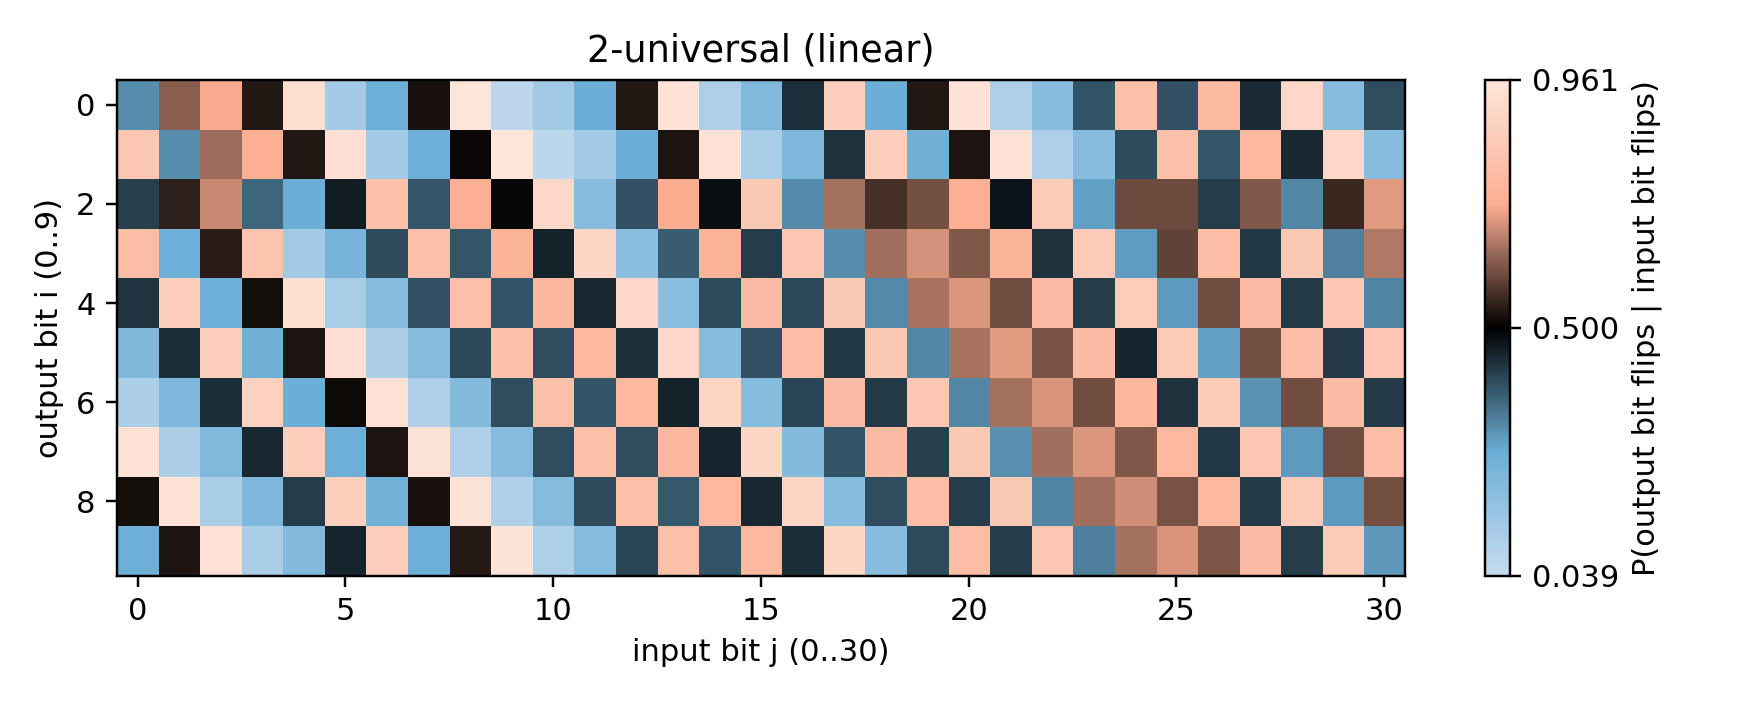
\includegraphics[width=\linewidth]{2univ_linear_heatmap.png}
    \caption{2-universal (linear)}
    \label{fig:q1-2univ}
  \end{subfigure}
  \hfill
  \begin{subfigure}[b]{0.48\linewidth}
    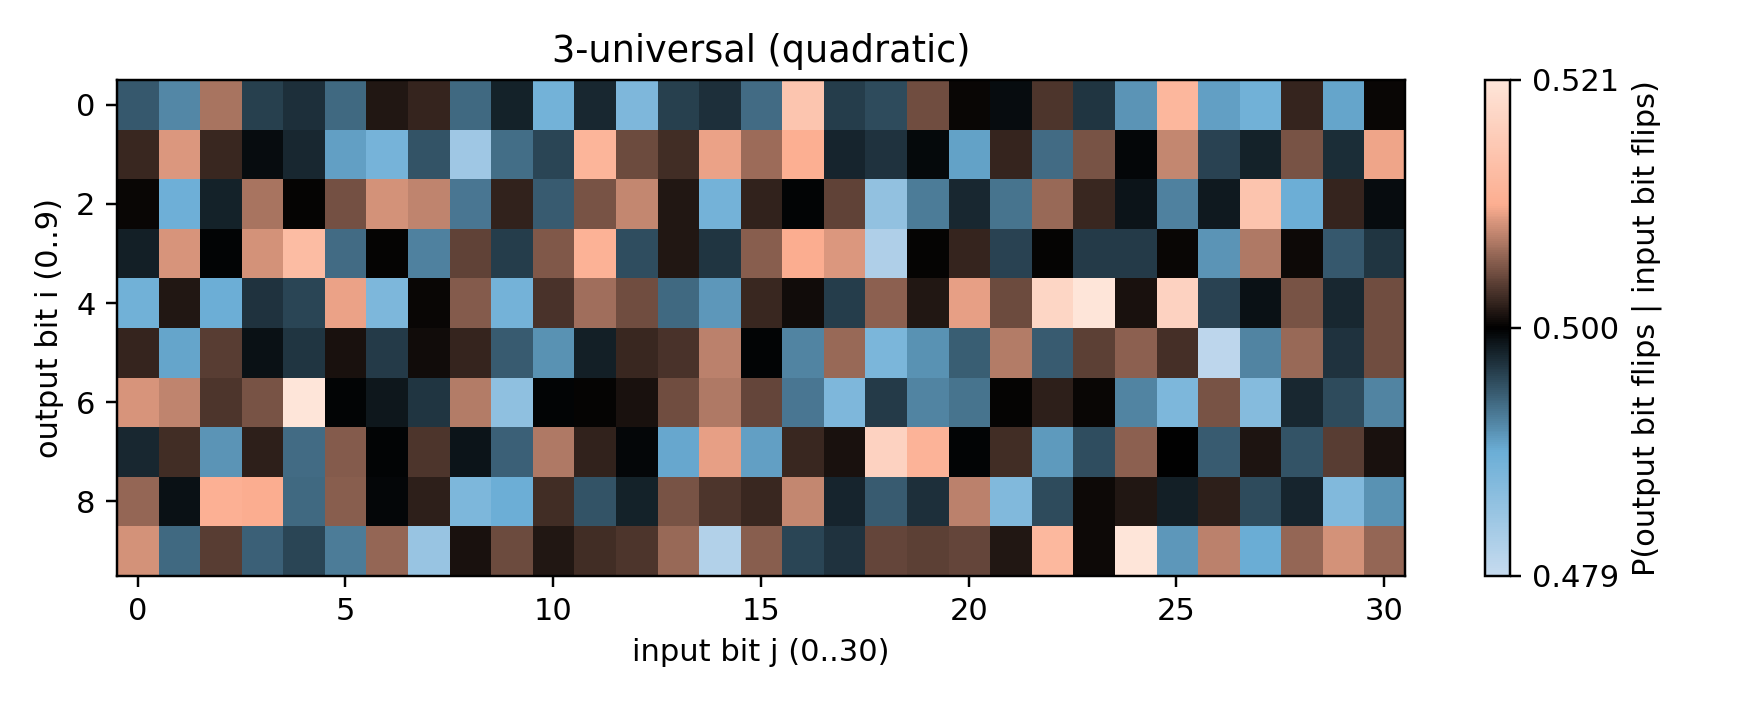
\includegraphics[width=\linewidth]{3univ_quadratic_heatmap.png}
    \caption{3-universal (quadratic)}
    \label{fig:q1-3univ}
  \end{subfigure}

  \vspace{0.6em}

  % Row 2
  \begin{subfigure}[b]{0.48\linewidth}
    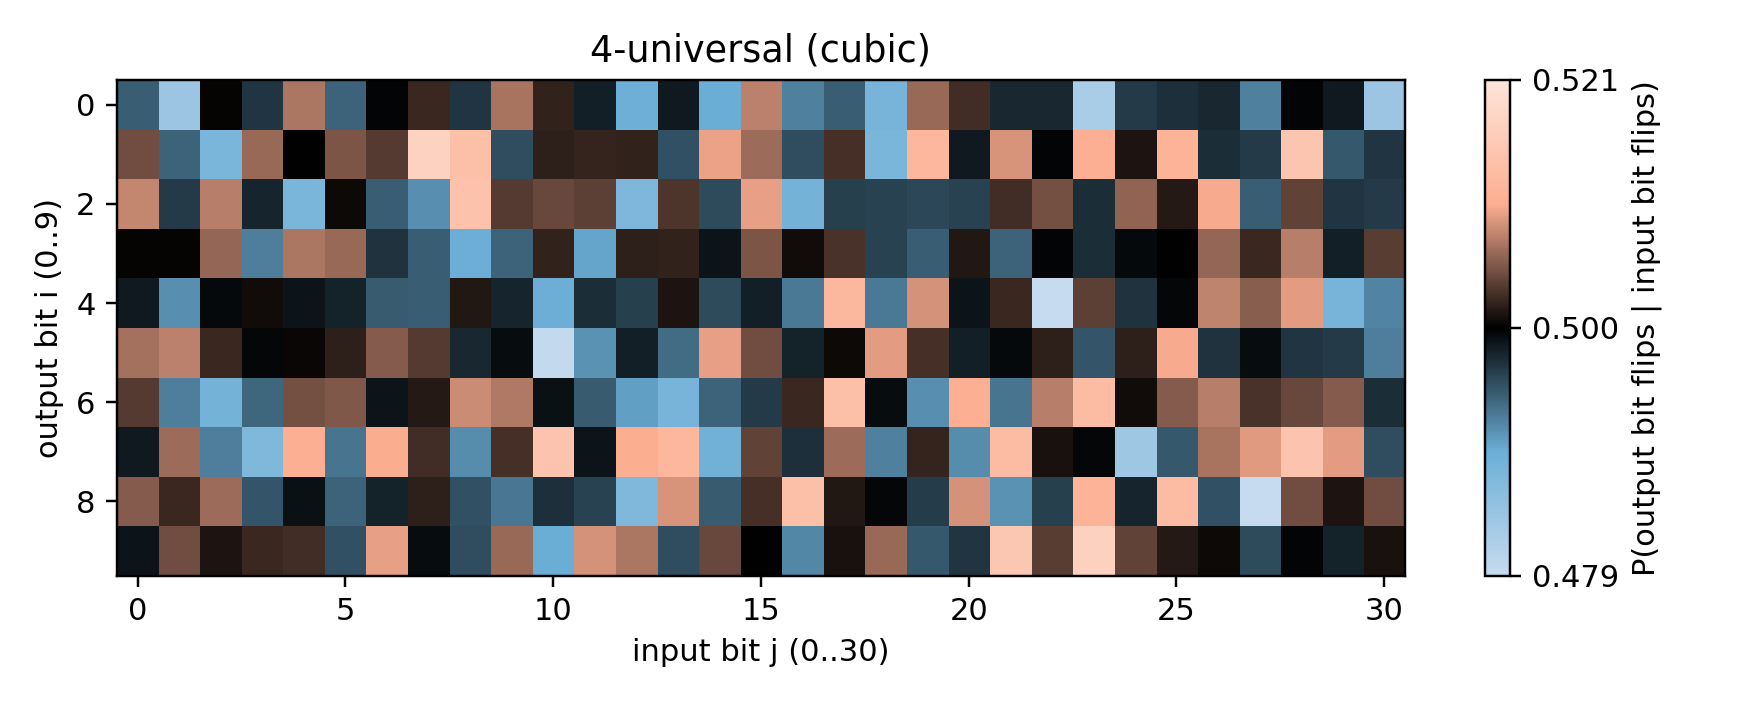
\includegraphics[width=\linewidth]{4univ_cubic_heatmap.png}
    \caption{4-universal (cubic)}
    \label{fig:q1-4univ}
  \end{subfigure}
  \hfill
  \begin{subfigure}[b]{0.48\linewidth}
    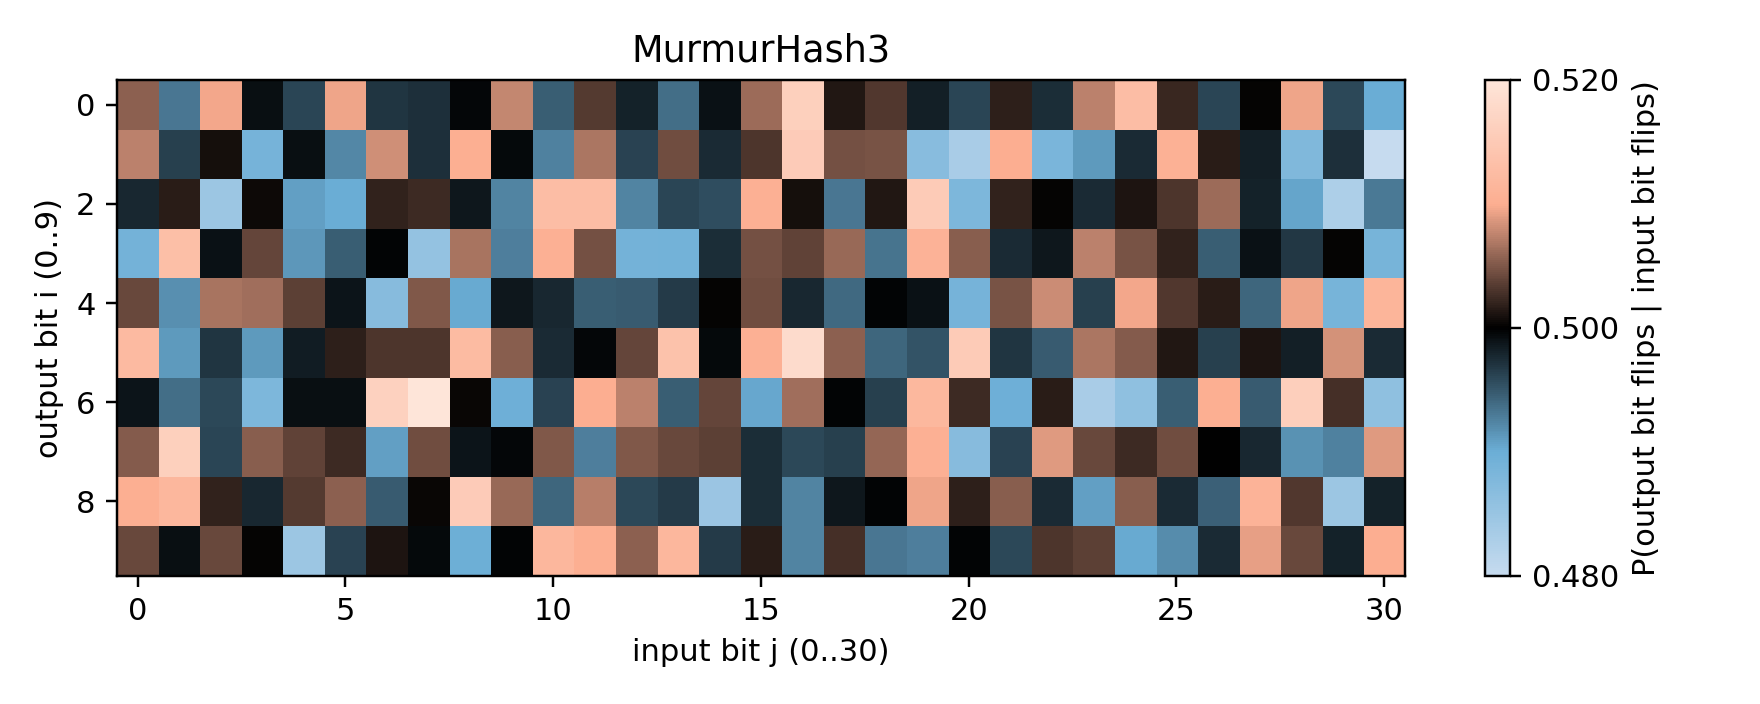
\includegraphics[width=\linewidth]{murmurhash3_heatmap.png}
    \caption{MurmurHash3}
    \label{fig:q1-murmur}
  \end{subfigure}

  \caption{Avalanche heatmaps ($10\times 31$). Color scale is centered at $0.5$ (black), so lighter indicates deviation from $0.5$.}
  \label{fig:q1-heatmaps}
\end{figure}

\paragraph{Interpretation}
As expected, \(h_2\), \(h_3\), and MurmurHash3 exhibit near-ideal avalanche (entries close to \(0.5\) with small spread). The 2-universal linear hash is \emph{not} avalanche: some output bits change almost deterministically for certain input-bit flips, while others rarely change. This is consistent with lower-independence families offering weaker bit-mixing, while higher-degree polynomials and practical non-cryptographic hashes like MurmurHash3 provide better diffusion.

\newpage
\section{Counting Turtle Confidence}
\textbf{Goal} Using Chebyshev’s inequality, I (i) give an explicit “constant$\times$std” band for the sample mean $\bar M$ of overlap counts, (ii) show how to choose $R$ so that the relative error $|\bar M-\mathbb{E}[M]|\le f\,\mathbb{E}[M]$ holds with failure probability at most $0.05$, (iii) translate the band into an interval for $\hat n=\frac{k_1k_2}{\bar M}$, and (iv) note when estimation is hard.

\paragraph{Setup} I repeat the same experiment $R$ times and observe the i.i.d. counts $M_1,\dots,M_R$. Let
\[
\bar M=\frac{1}{R}\sum_{i=1}^R M_i,
\qquad
\mu\triangleq \mathbb{E}[M]=\frac{k_1k_2}{n}
\]
The usual estimator of population size is $\hat n=\dfrac{k_1k_2}{\bar M}$.

\paragraph{Chebyshev band (“constant $\times$ std”)}
Because $\mathrm{Var}(\bar M)=\mathrm{Var}(M)/R$, Chebyshev gives, for any $\delta\in(0,1)$,
\[
\Pr\!\big[\,|\bar M-\mu|\ge a\,\big]\;\le\; \frac{\mathrm{Var}(M)}{R\,a^2}.
\]
Choosing
\[
\,a(\delta,R)=\sqrt{\frac{\mathrm{Var}(M)}{R\,\delta}}
=\frac{1}{\sqrt{\delta}}\underbrace{\sqrt{\frac{\mathrm{Var}(M)}{R}}}_{\mathrm{std}(\bar M)}\,
\]
ensures $\Pr[|\bar M-\mu|\le a]\ge 1-\delta$. For the assignment’s $\delta=0.05$,
\[
\,a=4.4721\;\sqrt{\frac{\mathrm{Var}(M)}{R}}\,
\]

\paragraph{Exact model vs.\ binomial approximation}
With sampling \emph{without} replacement, $M$ is hypergeometric:
\[
M\sim \mathrm{Hypergeometric}(n,\,k_1,\,k_2),\quad
\mathbb{E}[M]=k_2\frac{k_1}{n},\quad
\mathrm{Var}(M)=k_2\frac{k_1}{n}\Bigl(1-\frac{k_1}{n}\Bigr)\frac{n-k_2}{n-1}
\]
Since $\frac{n-k_2}{n-1}\le 1$, the binomial variance $k_2p(1-p)$ with $p=\frac{k_1}{n}$ is an \emph{upper bound} on the true variance. Thus, bands and $R$-requirements derived under the binomial model are \emph{conservative} for the exact model.

\paragraph{How many repetitions $R$ for a target relative error $f$ with failure $\le 0.05$?}
Impose $|\bar M-\mu|\le f\,\mu$ with failure at most $\delta$. Set $a=f\,\mu$ and solve:
\[
\delta\;\ge\; \frac{\mathrm{Var}(M)}{R\,(f\mu)^2}
\quad\Longrightarrow\quad
\,R\;\ge\;\frac{\mathrm{Var}(M)}{\delta\,f^2\,\mu^2}\,
\]
Under the binomial upper bound (conservative),
\[
\,R\;\ge\;\frac{k_2\,p(1-p)}{\delta\,f^2\,(k_2p)^2}
=\frac{1-p}{\delta\,f^2\,k_2\,p}\,,
\qquad p=\frac{k_1}{n}
\]
At $\delta=0.05$ this specializes to $R\ge \dfrac{1-p}{0.05\,f^2\,k_2\,p}$.

\paragraph{Translating to an interval for $\hat n$}
Since $g(m)=\frac{k_1k_2}{m}$ is decreasing on $(0,\infty)$, the event
$\bar M\in[\mu-a,\mu+a]$ with $\mu>a$ implies
\[
\hat n \in \left[\frac{k_1k_2}{\mu+a},\;\frac{k_1k_2}{\mu-a}\right]
\]
Using $\mu=\frac{k_1k_2}{n}$ this can be written as
\[
\hat n \in \left[\,\frac{n}{1+\frac{a n}{k_1k_2}}\;,\;\frac{n}{1-\frac{a n}{k_1k_2}}\,\right]
\]
In practice $n$ is unknown; I use the plug-in $\hat \mu=\bar M$ (and $\hat p=\bar M/k_2$) inside $a$ to produce a data-driven CI.

\paragraph{When is estimation hard?}
If $p=\frac{k_1}{n}$ is very small (few overlaps), then $\mu=k_2p$ is small and $1/\bar M$ is unstable; Chebyshev is also loose in that regime. Practically, I either increase $k_1,k_2$ to raise $\mu$ or increase $R$ via the formula above (or both).

\newpage

\section{Inequalities: Linear Probing with 5-independence}
With load factor \(\alpha=m/n=1/3\), and assuming the following bound for the expected search cost in linear probing (given in the problem):
\[
  \mathbb{E}[\text{cost}] \;=\; \mathcal{O}(1)\sum_{s=1}^{\lfloor \log_2 n \rfloor} 2^s \cdot \Pr\big[B_s \ge 2\,\mathbb{E}[B_s]\big],
\]
Where \(B_s\) counts the number of inserted keys that hash into a fixed \emph{interval of length \(2^s\)} (a contiguous block of table positions), under a \emph{5-independent} hash function.

\paragraph{Goal} Prove this sum is bounded by a constant (independent of \(n\)).

\paragraph{Setup} Fix an interval \(I_s\) of length \(2^s\). Let
\[
  B_s \;=\; \sum_{i=1}^m X_i,\quad X_i=\mathbf{1}\{h(\text{key}_i)\in I_s\},\quad
  p_s=\Pr[X_i=1]=\frac{2^s}{n}
\]
Then \(\mu_s \triangleq \mathbb{E}[B_s]=m p_s=\alpha\, 2^s\) and \(\mathrm{Var}(B_s)=m p_s(1-p_s)\le \mu_s\).

\paragraph{Fourth moment under 5-independence (statement \& sketch).}
\emph{Statement.} Under 5-independence, mixed moments up to order four factorize, and
\[
\mathbb{E}\!\left[(B_s-\mu_s)^4\right] \;\le\; C_1\,\mu_s \;+\; C_2\,\mu_s^2
\;=\; \mathcal{O}(\mu_s+\mu_s^2),
\]
for absolute constants $C_1,C_2$ (when $\mu_s\ge 1$; the $\mu_s<1$ case is handled separately below).

\emph{Sketch.} Let $Y_i=X_i-p_s$ so $B_s-\mu_s=\sum_{i=1}^m Y_i$ with
$\mathbb{E}[Y_i]=0$, $\mathbb{E}[Y_i^2]=p_s(1-p_s)$, and $\mathbb{E}[Y_i^4]\le C_0 p_s$.
Expanding and using that odd mixed moments vanish,
\[
\mathbb{E}\big[(B_s-\mu_s)^4\big]
= \sum_i \mathbb{E}[Y_i^4] + 6\!\!\sum_{i<j}\! \mathbb{E}[Y_i^2 Y_j^2],
\]
and 5-independence yields $\mathbb{E}[Y_i^2 Y_j^2]=\mathbb{E}[Y_i^2]\mathbb{E}[Y_j^2]=p_s^2(1-p_s)^2$.
Hence
\[
\mathbb{E}\big[(B_s-\mu_s)^4\big] \;\le\; C_0 m p_s + 6\binom{m}{2}p_s^2
\;=\; \mathcal{O}(\mu_s+\mu_s^2),\quad \mu_s=mp_s=\alpha 2^s.
\]
Markov on the 4th power gives
\[
\Pr[B_s\ge 2\mu_s] \;\le\; \frac{\mathbb{E}[(B_s-\mu_s)^4]}{\mu_s^4}
\;\le\; \frac{C}{\mu_s^2} \;=\; \frac{C}{\alpha^2\,2^{2s}}
\]



where \(\mu_s=m p_s=\alpha 2^s\). Markov’s inequality on the 4th power then gives
\(\Pr[B_s\!\ge 2\mu_s]\le \mathbb{E}[(B_s-\mu_s)^4]/\mu_s^4 \le C/\mu_s^2\),
yielding the summable bound in the next step.


\paragraph{Summation}
From the fourth–moment bound we obtained
\[
\Pr[B_s \ge 2\mu_s] \;\le\; \frac{C}{\mu_s^2}
\;=\; \frac{C}{(\alpha 2^s)^2}
\;=\; \frac{C}{\alpha^2\,2^{2s}}
\]
Plugging into the given sum,
\[
\sum_{s=1}^{\lfloor\log_2 n\rfloor} 2^s \cdot \Pr[B_s \ge 2\mu_s]
\;\le\; \sum_{s=1}^{\infty} 2^s \cdot \frac{C}{\alpha^2\,2^{2s}}
\;=\; \frac{C}{\alpha^2}\sum_{s=1}^{\infty} 2^{-s}
\;=\; \frac{C}{\alpha^2}\cdot 1
\;=\; \mathcal{O}\!\left(\frac{1}{\alpha^2}\right)
\]
Since the load factor $\alpha=m/n$ is fixed by the assignment (here $\alpha=\tfrac13$), the right-hand side is a numerical constant independent of $n$; in fact it equals $9C$ when $\alpha=\tfrac13$. \newline

For the very small-mean regime $\mu_s=\alpha 2^s<1$ (i.e., $2^s<1/\alpha$), a crude bound
$\Pr[B_s\ge 2\mu_s]\le \Pr[B_s\ge 1]\le \mu_s$ gives the partial contribution
\[
\sum_{s:\,\mu_s<1} 2^s\cdot \mu_s
\;\le\; \sum_{s\le s_0} 2^s\cdot (\alpha 2^s)
\;=\; \alpha \sum_{s\le s_0} 2^{2s}
\;=\; \alpha\cdot \mathcal{O}\!\big(2^{2s_0}\big)
\;=\; \alpha\cdot \mathcal{O}\!\big((1/\alpha)^2\big)
\;=\; \mathcal{O}\!\Big(\frac{1}{\alpha}\Big),
\]
where $s_0=\lfloor \log_2(1/\alpha)\rfloor$ is constant when $\alpha$ is constant. Thus both parts
(of large and small $\mu_s$) are bounded by constants depending only on $\alpha$, and the expected
search cost is $\mathcal{O}(1)$ for $\alpha=\tfrac13$.


\newpage

\section{Implement and Test Bloom Filters }

\textbf{Goal}
\begin{itemize}
  \item \textbf{Warmup:} (i) A hash factory mapping integers to a power-of-two range, and (ii) a \texttt{BloomFilter} class that takes $(n,c)$ and stores bits in a packed bitmap (no boolean arrays). Build a 10{,}000-key membership set and, for targets $c\!\in\!\{0.01,0.001,0.0001\}$, report \emph{Theoretical FP} and \emph{Real FP} together with $(R,k)$.
  \item \textbf{Extended:} Parse unique URLs, insert all $N$, and with policy $k=\lfloor 0.7R/N\rfloor$ vary $R\in\{2^{19},2^{20},2^{21},2^{22}\}$ to (i) report empirical FP and memory, (ii) plot FP vs.\ memory (use $R/8$ on the $x$-axis), and (iii) compare memory against a Python \texttt{set} and the theoretical $R/8$, with a brief comment.
\end{itemize}

\subsection*{Warmup}
\emph{Setup} Membership: $10{,}000$ unique integers from $[10{,}000..99{,}999]$; test: $1000$ non-members $+$ $1000$ true members. For each target $c$, I round $R$ to a power of two; the “Theoretical $c$” below is computed \emph{after} rounding $R$.


\begin{table}[h]
  \centering
  \begin{tabular}{rrrrrr}
    \toprule
    Target $c$ & $R$ (bits) & $k$ & Theoretical $c$ & Empirical $c$ & Memory (bytes) \\
    \midrule
    0.01   & 131{,}072 &  9 & $1.84141\times 10^{-3}$ & 0.002 & 16{,}441 \\
    0.001  & 262{,}144 & 18 & $3.3908\times 10^{-6}$  & 0     & 32{,}825 \\
    0.0001 & 262{,}144 & 18 & $3.3908\times 10^{-6}$  & 0     & 32{,}825 \\
    \bottomrule
  \end{tabular}
  \caption{Warmup results (membership $10^4$, test $1000{+}1000$). Theoretical FP is the model prediction after rounding $R$ to a power of two.}
\end{table}
\subsection*{Extended}
\emph{Setup} I parsed the AOL file to unique URLs, inserted all $N$ into a Bloom filter, and varied $R\!\in\!\{2^{19},2^{20},2^{21},2^{22}\}$ with the required policy $k=\lfloor 0.7R/N\rfloor$. Then it was evaluated on $1000$ sampled members and $1000$ random strings as negatives. For each $(R,k)$, I report the \emph{empirical} FPR and Bloom bitmap size (via \verb|sys.getsizeof|), alongside the theoretical bit budget $R/8$. I also measured a Python \texttt{set} containing the same universe (constant across $R$).

\begin{table}[h]
  \centering
  \begin{tabular}{rrrrr}
    \toprule
    $R$ (bits) & $k$ & Emp.\ FPR & BF bytes (measured) & Theory $R/8$ (bytes) \\
    \midrule
     524{,}288  &  1 & 0.503 &  65{,}593 &   65{,}536 \\
   1{,}048{,}576 &  1 & 0.301 & 131{,}129 &  131{,}072 \\
   2{,}097{,}152 &  3 & 0.081 & 262{,}201 &  262{,}144 \\
   4{,}194{,}304 &  7 & 0.006 & 524{,}345 &  524{,}288 \\
    \bottomrule
  \end{tabular}
  \caption{Extended memory comparison.}
\end{table}

\noindent\textit{Python \texttt{set} footprint (independent of $R$):} 16{,}777{,}432 bytes.

\paragraph{Measurement note (Python \texttt{set}).}
For the Bloom bitmap, I reported the exact container size via \verb|sys.getsizeof(bytearray)|, which equals \(R/8\) plus a small fixed overhead.
For the Python \texttt{set}, I intentionally reported the \emph{container-only} size taken from \(\verb|sys.getsizeof(set)|\), which does \emph{not} include the memory of the stored elements
(e.g. strings) orheir internal allocations. This choice is conservative \emph{in favor of the set};
the true deep footprint (for example, by \texttt{ pimpler.asizeof} or summing \verb|sys.getsizeof| over all elements) is much larger for \(N\!\approx\!3.78\times 10^5\) URLs.
However, the Bloom vs. theory comparison is exact because it concerns only the bitmap bits.


\subsection*{Memory Usage Comparison}
\begin{itemize}
  \item \emph{Bloom vs theory:} Measured bitmap size matches $R/8$ up to a small constant overhead of $\approx57$ bytes in every setting ($\text{measured} - R/8 = 57$).
  \item \emph{Bloom vs Python hashtable:} At $R{=}4{,}194{,}304$ the Bloom bitmap uses $524{,}345$ bytes vs.\ \texttt{set} at $16{,}777{,}432$ bytes ($\sim32\times$ smaller); the ratio widens further at smaller $R$.
  \item \emph{Accuracy--memory tradeoff:} With $k=\lfloor 0.7R/N\rfloor$, empirical FPR falls from $0.503$ to $0.006$ as $R$ increases, while memory scales linearly with $R$ (the $R/8$ line).
\end{itemize}

\begin{figure}[h]
  \centering
  \begin{subfigure}[b]{0.32\linewidth}
    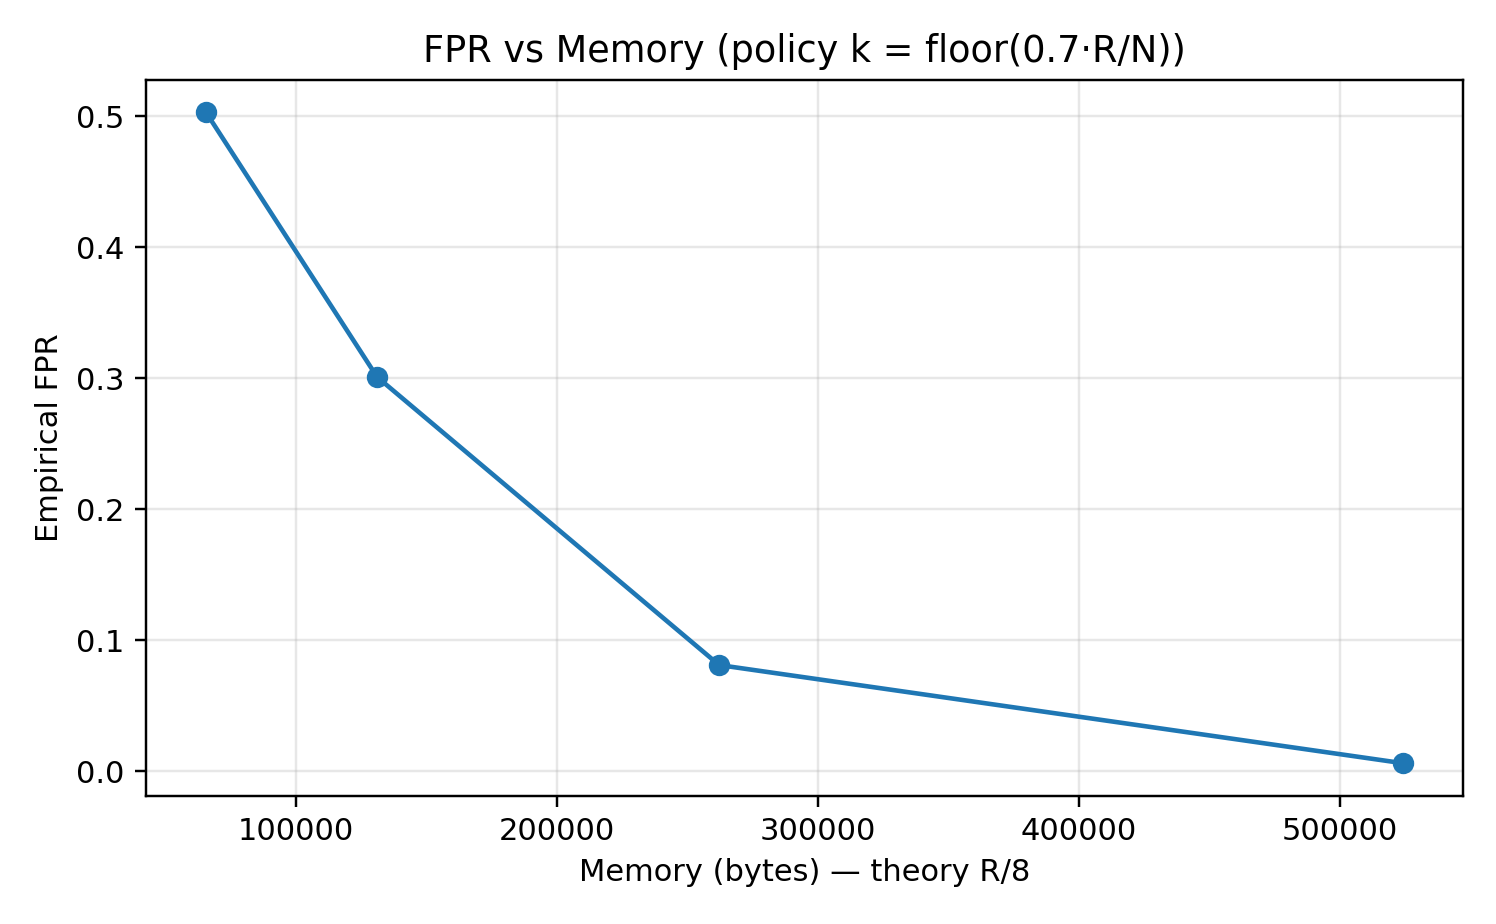
\includegraphics[width=\linewidth]{fpr_vs_memory.png}
    \caption{FPR vs memory ($R/8$).}
  \end{subfigure}
  \caption{Extended evaluation with policy $k=\lfloor 0.7\,R/N\rfloor$.}
\end{figure}


\paragraph{Conclusions}
Empirical FP decreases rapidly as $R$ grows and tracks theory. The packed bitmap’s measured size agrees with $R/8$ up to small object overhead, while a Python \texttt{set} is orders of magnitude larger for this $N$.

\newpage

\section*{Appendix A: How to Run}

\paragraph{Environment (Python \texorpdfstring{$\ge$}{≥} 3.9).}
\begin{enumerate}
  \item \textbf{(Recommended) Create a virtual environment}
\begin{verbatim}
python3 -m venv env

# This is MacOS Command. Do equivalent if on windows.
source env/bin/activate
\end{verbatim}

  \item \textbf{Install dependencies}
\begin{verbatim}
python -m pip install --upgrade pip
pip install -U numpy pandas matplotlib scikit-learn
\end{verbatim}
  % If shipping a requirements file, you can alternatively do:
  % \verb|pip install -r requirements.txt|.
\end{enumerate}

\paragraph{Dataset}
If you have the AOL file, place \texttt{user-ct-test-collection-01.txt}
in the working directory (or a \texttt{data/} subfolder). The Q4 script will attempt to
detect it automatically when \verb|--extended| is used. If the file is absent, the extended
run is skipped.

\paragraph{Commands.}
\begin{itemize}
  \item \textbf{All results:} \verb|python3 main.py --all|
  \item \textbf{Only Q1 (hash avalanche):} \verb|python3 main.py --q1|
  \item \textbf{Only Q4 (Bloom tests):} \verb|python3 main.py --q4| \quad
        (add \verb|--extended| to run the AOL dataset sweep if the file is present)
\end{itemize}

\paragraph{Outputs (where to find things).}
\begin{itemize}
  \item \textbf{Q1:} \texttt{outputs/q1/}
    \begin{itemize}
      \item Heatmaps: \texttt{2univ\_linear\_heatmap.png}, \texttt{3univ\_quadratic\_heatmap.png},\\
            \texttt{4univ\_cubic\_heatmap.png}, \texttt{murmurhash3\_heatmap.png}
      \item Deviation heatmaps: corresponding \texttt{*\_dev\_heatmap.png}
      \item CSVs: \texttt{*\_avalanche.csv}; summary: \texttt{summary.txt}
    \end{itemize}
  \item \textbf{Q4:} \texttt{outputs/q4/}
    \begin{itemize}
      \item Warmup table dump: \texttt{Results.txt} and \texttt{results.csv}
      \item Memory reports: \texttt{memory.txt} (warmup), \texttt{extended\_memory.txt} (AOL)
      \item Extended sweep: \texttt{extended.csv} (AOL metrics)
      \item Plots: \texttt{fpr\_vs\_memory.png}
    \end{itemize}
\end{itemize}

\paragraph{Reproducibility.}
All scripts are deterministic given the fixed seeds listed in the paper’s “Constants” section.
Running the commands above will regenerate the CSVs and figures in the same paths.


\section*{Appendix B: Submitted Code Artifacts}
Per the instructions, all code is provided as compressed archives rather than embedded listings here.

\begin{itemize}
  \item \textbf{Source zip:} \texttt{src.zip} containing the files \texttt{main.py}, \texttt{q1\_avalanche.py}, \texttt{q4\_bloom.py}, \texttt{q1\_heatmaps.py}, \texttt{q4\_plots.py}.
  \item \textbf{Outputs zip:} \texttt{outputs.zip} containing all CSVs, text summaries, and figures produced by running the scripts.
\end{itemize}


\end{document}
